\documentclass{article}
%%%%%%%%%%%%%%%%%%%%%%%%%%%%% Define Article %%%%%%%%%%%%%%%%%%%%%%%%%%%%%%%%%%
%%%%%%%%%%%%%%%%%%%%%%%%%%%%%%%%%%%%%%%%%%%%%%%%%%%%%%%%%%%%%%%%%%%%%%%%%%%%%%%

%%%%%%%%%%%%%%%%%%%%%%%%%%%%% Using Packages %%%%%%%%%%%%%%%%%%%%%%%%%%%%%%%%%%
\usepackage{float}
\usepackage[letterpaper,portrait]{geometry}
\usepackage{graphicx}
\usepackage{anysize}
\usepackage{lipsum}
\usepackage{amsmath,amssymb,amsthm}
\usepackage[utf8]{inputenc}
\usepackage{multirow}
\usepackage{csquotes}
\usepackage[spanish]{babel}
\usepackage{apacite}
\usepackage{multicol}
\usepackage{parskip}
\usepackage{setspace}
\usepackage{empheq}
\usepackage{mdframed}
\usepackage{booktabs}
\usepackage{lipsum}
\usepackage{graphicx}
\usepackage{color}
\usepackage{psfrag}
\usepackage{pgfplots}
\usepackage{bm}
\usepackage{tocloft}

%%%%%%%%%%%%%%%%%%%%%%%%%%%%%%%%%%%%%%%%%%%%%%%%%%%%%%%%%%%%%%%%%%%%%%%%%%%%%%%

% Other Settings

%%%%%%%%%%%%%%%%%%%%%%%%%% Page Setting %%%%%%%%%%%%%%%%%%%%%%%%%%%%%%%%%%%%%%%
\geometry{letterpaper, margin=2.54cm}

%%%%%%%%%%%%%%%%%%%%%%%%%% Define some useful colors %%%%%%%%%%%%%%%%%%%%%%%%%%
\definecolor{ocre}{RGB}{243,102,25}
\definecolor{mygray}{RGB}{243,243,244}
\definecolor{deepGreen}{RGB}{26,111,0}
\definecolor{shallowGreen}{RGB}{235,255,255}
\definecolor{deepBlue}{RGB}{61,124,222}
\definecolor{shallowBlue}{RGB}{235,249,255}
%%%%%%%%%%%%%%%%%%%%%%%%%%%%%%%%%%%%%%%%%%%%%%%%%%%%%%%%%%%%%%%%%%%%%%%%%%%%%%%

%%%%%%%%%%%%%%%%%%%%%%%%%% Define an orangebox command %%%%%%%%%%%%%%%%%%%%%%%%
\newcommand\orangebox[1]{\fcolorbox{ocre}{mygray}{\hspace{1em}#1\hspace{1em}}}
%%%%%%%%%%%%%%%%%%%%%%%%%%%%%%%%%%%%%%%%%%%%%%%%%%%%%%%%%%%%%%%%%%%%%%%%%%%%%%%

%%%%%%%%%%%%%%%%%%%%%%%%%%%% English Environments %%%%%%%%%%%%%%%%%%%%%%%%%%%%%
\newtheoremstyle{mytheoremstyle}{3pt}{3pt}{\normalfont}{0cm}{\rmfamily\bfseries}{}{1em}{{\color{black}\thmname{#1}~\thmnumber{#2}}\thmnote{\,--\,#3}}
\newtheoremstyle{myproblemstyle}{3pt}{3pt}{\normalfont}{0cm}{\rmfamily\bfseries}{}{1em}{{\color{black}\thmname{#1}~\thmnumber{#2}}\thmnote{\,--\,#3}}
\theoremstyle{mytheoremstyle}
\newmdtheoremenv[linewidth=1pt,backgroundcolor=shallowGreen,linecolor=deepGreen,leftmargin=0pt,innerleftmargin=20pt,innerrightmargin=20pt,]{theorem}{Theorem}[section]
\theoremstyle{mytheoremstyle}
\newmdtheoremenv[linewidth=1pt,backgroundcolor=shallowBlue,linecolor=deepBlue,leftmargin=0pt,innerleftmargin=20pt,innerrightmargin=20pt,]{definition}{Definition}[section]
\theoremstyle{myproblemstyle}
\newmdtheoremenv[linecolor=black,leftmargin=0pt,innerleftmargin=10pt,innerrightmargin=10pt,]{problem}{Problem}[section]
%%%%%%%%%%%%%%%%%%%%%%%%%%%%%%%%%%%%%%%%%%%%%%%%%%%%%%%%%%%%%%%%%%%%%%%%%%%%%%%

%%%%%%%%%%%%%%%%%%%%%%%%%%%%%%% Plotting Settings %%%%%%%%%%%%%%%%%%%%%%%%%%%%%
\usepgfplotslibrary{colorbrewer}
\pgfplotsset{width=8cm,compat=1.9}
%%%%%%%%%%%%%%%%%%%%%%%%%%%%%%%%%%%%%%%%%%%%%%%%%%%%%%%%%%%%%%%%%%%%%%%%%%%%%%%

%%%%%%%%%%%%%%%%%%%%%%%%%%%%%%% Title & Author %%%%%%%%%%%%%%%%%%%%%%%%%%%%%%%%
\author{Gustavo Vergara}
%%%%%%%%%%%%%%%%%%%%%%%%%%%%%%%%%%%%%%%%%%%%%%%%%%%%%%%%%%%%%%%%%%%%%%%%%%%%%%%


\begin{document}
\pgfplotsset{compat=1.18}
\setstretch{2}

\begin{titlepage}
    \centering
    
    
    \vspace{3cm}
    {\scshape \Large Planteamiento de ecuación. - GA2-240201528-AA2-EV01 \par}
    \vspace{6cm}
    \textbf\large\scshape{\par}
         \vspace{0.5cm}
         
    {\Large Vergara Pareja Gustavo\par}
    \vspace{6cm}
    {\scshape\Large Fabiola Perez\par}
    \vspace{0.5cm}
    {\scshape\Large Tecnología en Análisis y Desarrollo de Software \par}
    \vspace{0.5cm}
    {\scshape\Large SENA - Centro Agropecuario Regional Cauca\par}
    \vspace{0.5cm}
    {\Large \today \par}
    \end{titlepage}

\begin{flushleft}
    \large \textbf{EVIDENCIA A SOLUCIONAR}\\
    \vspace{0.5cm}
    \section*{Evidencia GA2-240201528-AA2-EV01: planteamiento de ecuación}
Para esta evidencia, se toma como estrategia el aprendizaje basado en problemas, en el cual usted resolverá un problema de aplicación utilizando las herramientas matemáticas propuestas en el material de formación del componente medio.
\newline
\large \textbf{Problema de aplicación}\\
Una firma de arquitectos en una estrategia de mercadeo muy innovadora busca entregar a cada uno de sus clientes una casa en escala de chocolate, como la que se ve en la siguiente figura.
La repostería que contrataron para llevar a cabo dicho proyecto tiene dos inconvenientes. El primero es el uso óptimo de la materia prima en el diseño de las casas; y el segundo es encontrar una opción económicamente viable para el empaque de la casa, pues al ser comestible debe estar protegida con una vitrina de metacrilato.
Se solicita que, para aportar a la solución de esta situación, realice lo siguiente:

    \begin{itemize}
        \item a. Plantee una ecuación que represente el área total de la casa de chocolate.
        \item b. Busque una función que represente el costo total de una casa de chocolate vs. cantidad de casas de chocolate. Para esto debe tener en cuenta que hay unos gastos fijos como el costo de la materia prima, el salario de los reposteros, costo del material de la vitrina en la que se entregará la casa, entre otros.
        \item c. Proponga una solución más rentable para la entrega de casas de chocolate.
        \item d. Plasmar estos resultados en un documento donde justifique la solución que le dio al problema.
         \end{itemize} 
    \end{flushleft}
    \newpage
    \tableofcontents
    \newpage
\section{Ecuación del área total}
\begin{figure}[H]
    \centering
    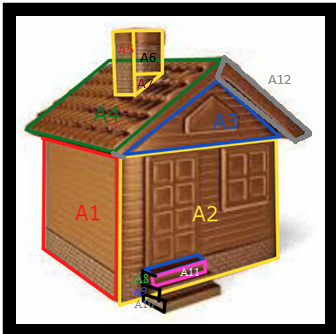
\includegraphics[width=0.6\textwidth]{CASA3.png}
    \caption{Casa de chocolate}
    \label{fig:imagen1}
    \end{figure}

\begin{figure}[H]
    \centering
    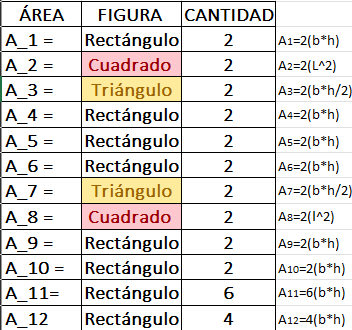
\includegraphics[width=0.6\textwidth]{2.png}
    \caption{Áreas de la casa}
    \label{fig:imagen1}
    \end{figure}
Sabiendo que b y h y l, son distintos para cada área, entonces la ecuación que representa el área total será:
\begin{figure}[H]
    \centering
    
\includegraphics[width=0.6\textwidth]{1.png}
    
    \label{fig:imagen1}
    \end{figure}
    Cada figura de la casa genera un área distinta en función de sus dimensiones.\newline
Nota: El área calculada es el área superficial de la casa.

\section{Ecuación del área total de la vitrina}

Suponiendo que toda la vitrina formará un cubo de metacrilato el área total será:
\newline
\begin{figure}[H]
    \centering
    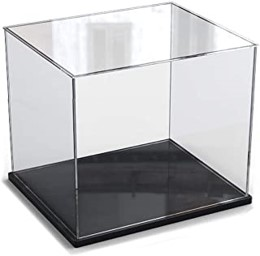
\includegraphics[width=0.3\textwidth]{3.jpg}
    \caption{Vitrina}
\end{figure}

\begin{equation}
    A_{total}= 6 \cdot L  ^{2}
\end{equation}
Cabe resaltar que para un metro cuadrado de metacrilato, L debe ser menor a 0.4082 m
\newpage
\section{Función de costo}

\text{Para los costos fijos tendremos en cuenta:}
\begin{itemize}
\item \text{Materia prima}
\item \text{Salario de repostero}
\item \text{Costo de metacrilato por 1 vitrina}
\end{itemize}
Para 1 casa de chocolate se utilizará:
\begin{itemize}
    \item \text{1 Base de chocolate = 1 Kilogramo = \$35600}
    \item \text{1 repostero (por 6 horas) = \$72000}
    \item \text{1 m2 de metacrilato = \$135000}
    \end{itemize}
\text{Costo fijo por unidad} = 35600+72000+135000 = \$242600

\text{Función de costo}
\begin{equation}
    C(x) = 242600 \cdot x
\end{equation}

\section{Resultados de los costos totales para la entrega de las casas}
Con la función de costos procedemos a hallar el costo total para crear 75 casas de chocolate: 

C(X)=242600(X)
C(75) = 242600 (75) = \$18 195 000

Así entonces, el costo total será de \$18 195 000 por 75 casas.
\section{Propuesta de mejora}
Para mejorar la rentabilidad, hay pocas opciones:
\begin{itemize}
    \item Disminuir las dimensiones de la casa de chocolate y por ende su volumen. Por lo que el metacrilato también disminuirá.
    \item Cambiar la mano de obra por una programable.
\end{itemize}
\section{Conclusiones}
En conclusión, la actividad en el calculo de áreas fué con dimensiones indicadas y ayudo a desarrollar el pensamiento de área superficial.

\bibliographystyle{apacite}
\nocite{*}
\bibliography{referenciados}
\end{document}